\documentclass[a4paper]{article}

\usepackage{babel}
\usepackage[latin1]{inputenc}
\usepackage{amssymb}
\usepackage{framed}
\usepackage{graphicx}

\setlength{\parindent}{0pt}
\setlength{\parskip}{3ex}

\begin{document}

\begin{center}
  {\large Artificial Neural Networks and Deep Architectures, DD2437}\\
  \vspace{7mm}
  {\huge Short report on lab assignment 2\\[1ex]}
  {\Large Radial basis functions, competitive learning and self-organisation}\\
  \vspace{8mm}  
  {\Large Rakin Ali, Steinar Logi and Hasan \textbf{Efternamn}\\}
  \vspace{4mm}
  {\large January,08 2023\\}
\end{center}

\section{Main objectives and scope of the assignment}

Our major goals in the assignment were  
\begin{itemize}
\item To build, design and analyze a RBF network 
\item To understand Vector Quantization and how to implement it  
\item To implement Self organising maps in order to understand the underlying theory behind it
\end{itemize}

\section{Methods} All parts of the labs were implemented twice just to be safe. Everything was written in Python 3.9 and all plots were done with Matplotlib. 

\section{Results and discussion - Part I: RBF networks and Competitive Learning \normalsize{\textit{(ca. 2.5-3 pages)}}}


\subsection{Function approximation with RBF networks\\ \normalsize{\textit{(ca. 1.5-2 pages)}}}
\textit{Combine results and findings from RBF simulations on both noise-free and noisy function approximation (sin(2x) and square (2x)). Try to organise them into subsections, and please make sure you pay attention to the comparison between RBF- and MLP-based approaches as well as the comparative analyses of batch and on-line learning schemes. Answer the questions, quantify the outcomes, discuss your interpretations and summarise key findings as conclusions.}


We performed function approximation with Radial basis function networks. The functions we approximated were the $sin(2x)$ and $square(2x)$ functions. The training set for the functions was obtained by using the domain $[0:2\pi]$. The step size was 0.1 and we sampled both the functions to obtain the training set. For the test set we started from 0.05 and used the same step size. The networks were trained using batch mode. The two function that we approximated can be seen in figure \ref{fig:two-functions}\\

\begin{figure}
    \centering
    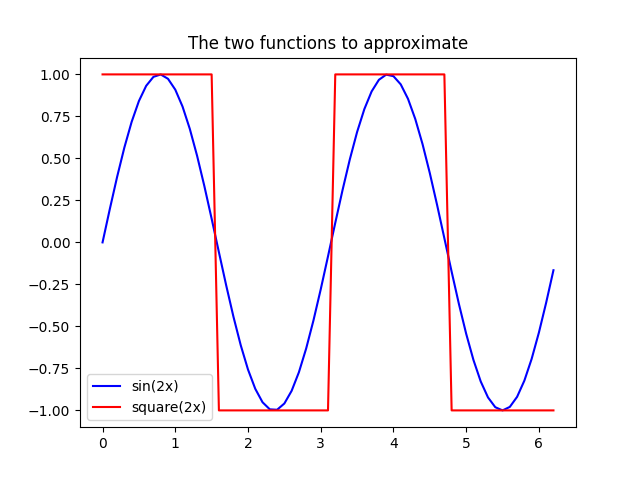
\includegraphics[width=0.4\textwidth]{Labs/Lab 2/Steinar/results/two-functions.png}
    \caption{The two functions}
    \label{fig:two-functions}
\end{figure}

When fitting the radial basis function network to the sine function we discovered that it was enough to use only 4 units to be able to obtain an error below 0.1 and to obtain an error below 0.01 it was enough to use 6 units. When using 4 units we placed them at each minimum and maximum of the sine wave in the interval $[0:2\pi]$. When we used 6 neurons we placed the units at each minimum and maximum and then we placed two neurons at the ends of the interval. \\

When we fitted the $square(2x)$ function we observed that if we used the $sgn(y)$ activation function in the output layer we could reduce the error to zero. The $sgn(y)$ returns 1 if the input, $y$, is greater or equal to zero and -1 if the input is less than zero. The width of the radial basis functions was 2. This approximated function can be seen in figure \ref{fig:square-non} 



\subsection{Function approximation with noise data}
We performed function approximations for $sin(2x)$ and $square(2x)$ using training and testing data subsets containing noise to see how RBF models perform and discover patterns although noise. In addition, we compared the performance of various RBF networks to understand how different parameters can affect the performance of the models. Furthermore, two different approached were implemented to train the RBF networks, the delta rule and the least square

\begin{figure} 
     \centering
     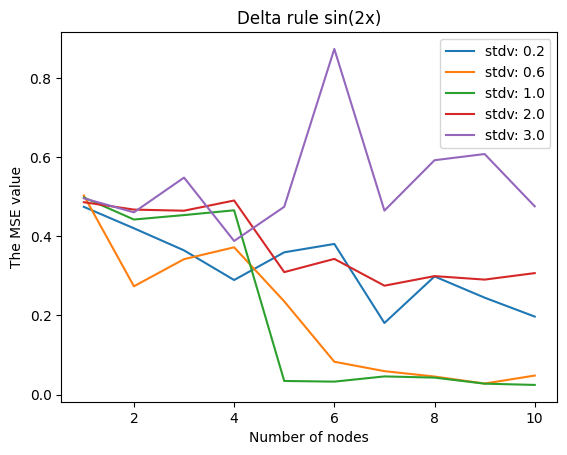
\includegraphics[width=0.6\textwidth]{Labs/Lab 2/figures/3.2/MSE_sin(2x)_delta.png}
     \caption{The MSE error with delta rule implementation}
     \label{fig:sin(2x)}
\end{figure}

\begin{figure} 
     \centering
     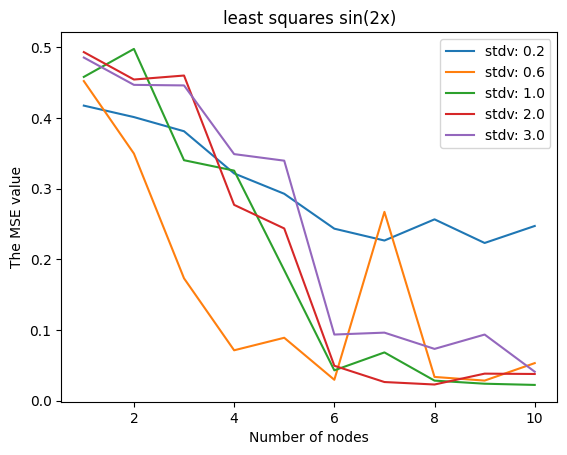
\includegraphics[width=0.6\textwidth]{Labs/Lab 2/figures/3.2/MSE_sin(2x)_least.png}
     \caption{The MSE error with least square implementation}
     \label{fig:sin(2x)}
\end{figure}

Increasing the network's nodes improves the generalization performance, which can be seen in both implementations. However, a too low width, such as 0.2, will give low accuracy.
A higher width than 1 seems only to worsen the generalization performance in the delta rule implementation.\ref{fig:sin(2x)} 


Choosing 





\subsection{Competitive learning for RBF unit initialisation\\ \normalsize{\textit{(ca. 1 page)}}}
\textit{Please refer first to the results in the previous section, i.e. those obtained without any automated initialisation. Then in the next subsection focus on two-dimensional regression with RBF networks.}

In this part of the assignment we used competitive learning to initialize the weights. We tried using competitive learning to initialize the weights used in the RBF network that was trained on the training set from the $sin(2x)$ function. The weights for this training set are of course one dimensional. We can therefore visualize the weights by drawing the output from the competitive learning on the x axis in a two dimensional graph. The results can be seen in figure \ref{fig:cl}. The image on the left shows the function obtained with RBF network trained on the $sin(2x)$ dataset without noise and the image on the right shows the function obtained with the RBF network trained on the $sin(2x)$ dataset with noise. On both images the weights obtained from the competitive learning can be seen as the orange dots on the x-axis. The width of the rbf nodes was the number of weights divided by the domain of the function or $2\pi$ in both cases. When we tried this using 6 nodes we obtained a worse results than when we manually placed the weights in the weight space but still the results were pretty good. The absolute relative error for the function with noise was around 0.104 so the network seems to generalize pretty well. 






\section{Results and discussion - Part II: Self-organising maps \normalsize{\textit{(ca. 2 pages)}}}

\subsection{Topological ordering of animal species}
\begin{figure} [htb]
    \centering
    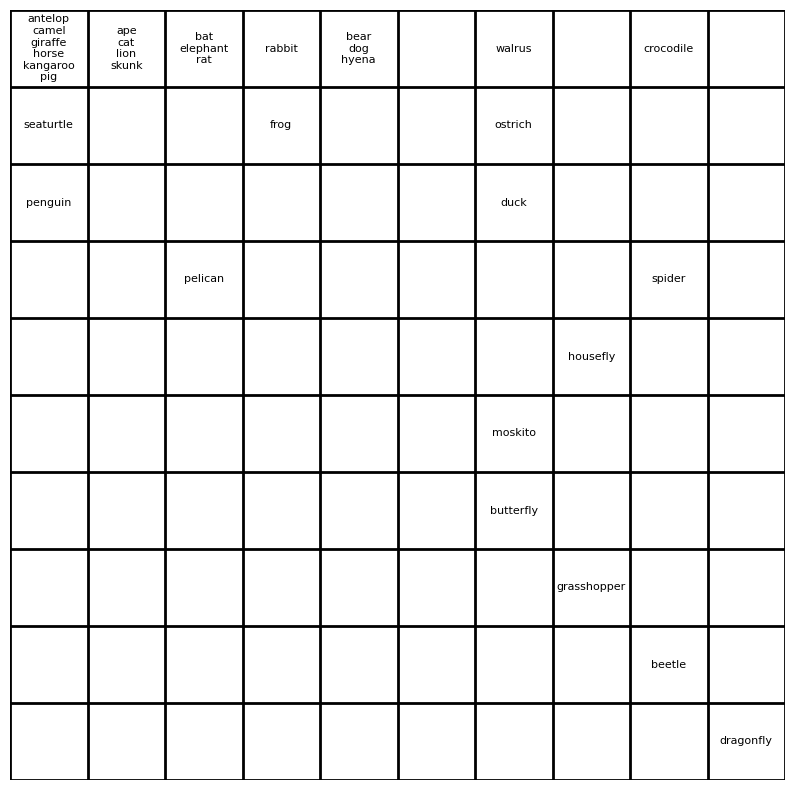
\includegraphics[width=5cm]{Labs/Lab 2/Results/animal_som.png}
    \caption{Animals sorted in 100 size nodes}
    \label{fig:SOM_animals}
\end{figure}
In the code we set the initial neighbors to 50, had 1000 epochs and a learning rate of 0.2 as in the instructions. The figure can be seen in \ref{fig:SOM_animals}. The figure makes sense as cat and lion are matched together and with closer observation you'll notice how most insects are grouped together. However they are certain places where it does not entirely make sense, specifically between frog, ape and walrus. In general it made sense. 



\subsection{Cyclic tour}
Figure \ref{fig:SOM_cycle} represents the shortest cycling tour which passes through all the cities based on their coordinates. We got different paths whenever we ran the code. The dotted lines represent which city is closest to that node as in certain times the nodes were placed between two cities.  
\begin{figure}[htb]
    \centering
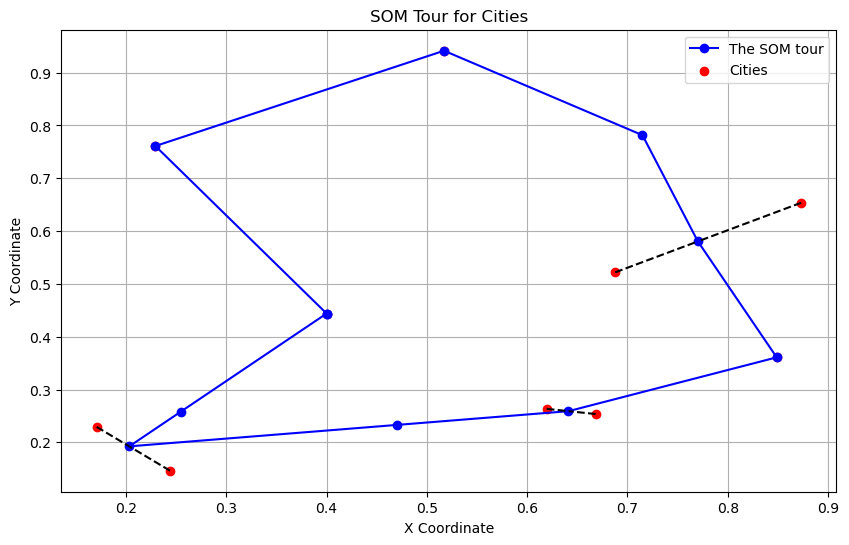
\includegraphics[width=7.5cm]{Labs/Lab 2/Results/Cyclic_som.png}
    \caption{Best path by SOM network}
    \label{fig:SOM_cycle}
\end{figure}

\subsection{Clustering with SOM}
\begin{figure}[htb]
    \centering
    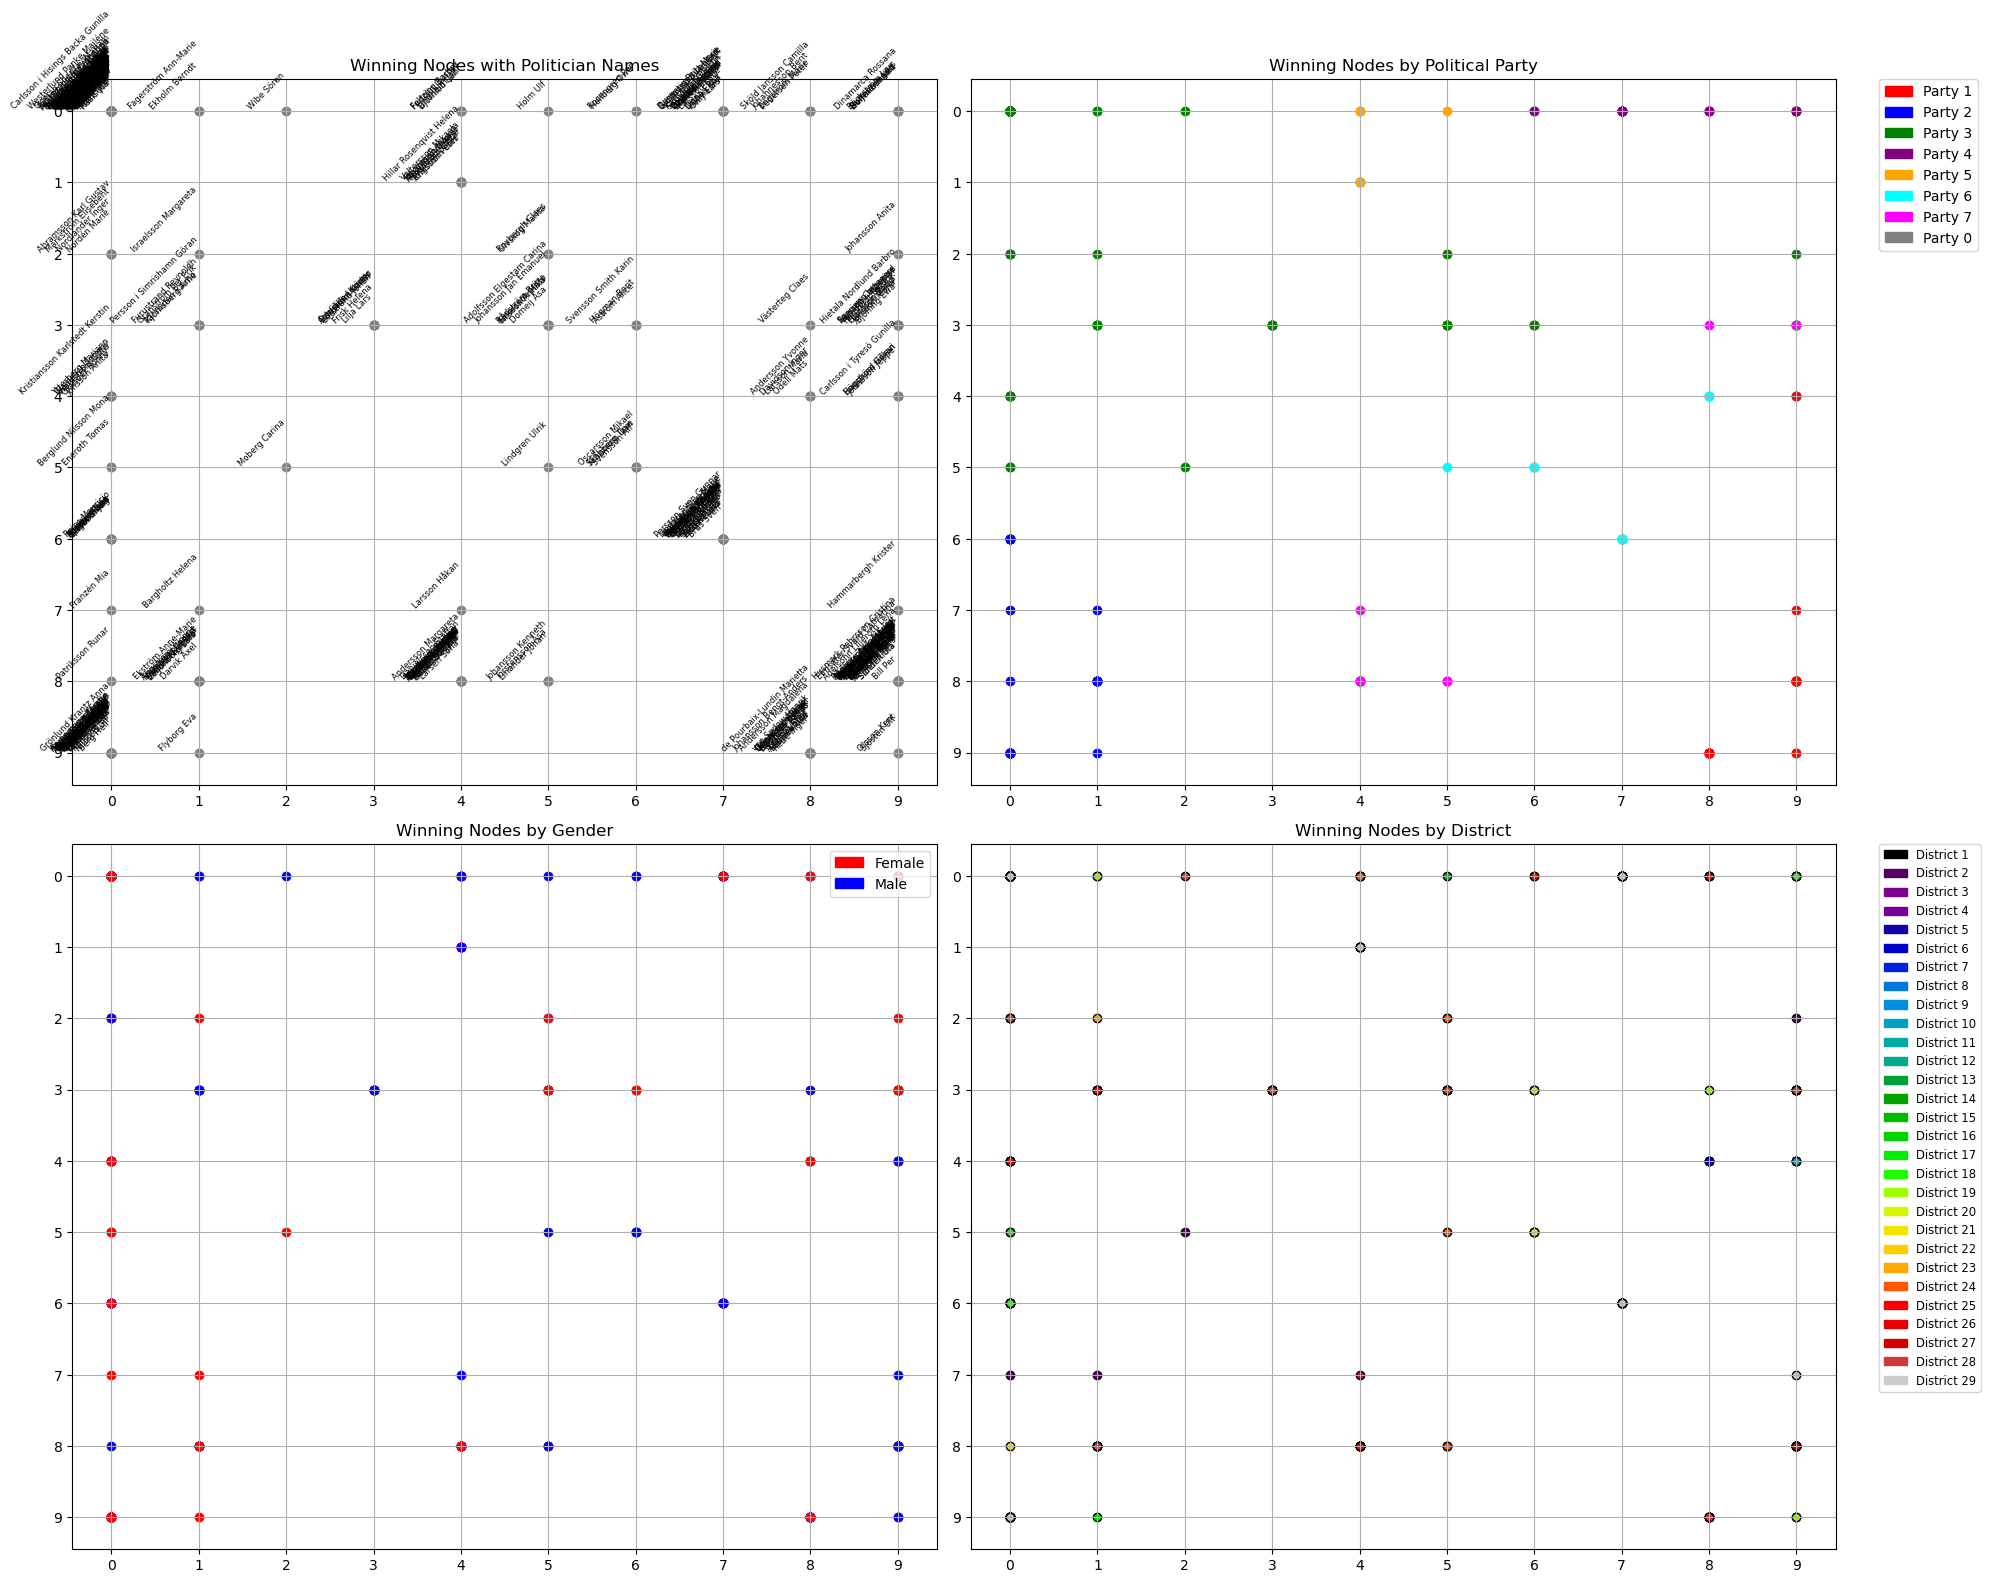
\includegraphics[width=\textwidth]{Labs/Lab 2/Results/politics_som.png}
    \caption{SOM grid based on political data}
    \label{fig:SOM_politics}
\end{figure}
In this assignment we were given a dataset on how 349 politicians voted on 31 separate decision and we were given their political party, gender, name and district. The results can be figure \ref{fig:SOM_politics}. In the subfigure at the top left, we to see the names of each 349 politicians and how similar they are to each other. On the figure to the top right, we see how similar each politician voted based on their political party and notice how closely most of them are to each other. The blue, red and green are tend to stick close to each together. Regarding district and gender, there is little there are no observable pattern. 




\section{Final remarks \normalsize{\textit{(max 0.5 page)}}}
\textbf{I'll write this once you are all done with adding images and so on. Hassan you'll need to fill in for RBF}

\end{document}
